%!TEX encoding = IsoLatin

%% Document is article 
\documentclass[a4paper]{article}

%% ----------------------------------------------------- PACKAGES ----------------------------------------------------- %%
\usepackage{coolArticle}

%% ---------------------------------------------------- DOCUMENT ---------------------------------------------------- %%
\begin{document}

\noindent \textsc{Gallos-Montbrun} Gr�goire\\
\textsc{Faury} Louis 
	\titlebox{0.6}{Model Predictive Control}{Exercice \#5 - \textcolor{blue}{Group 2}}
	
	\vspace{10pt}
	\paragraph{} We consider the following system : 
	\begin{equation}
		\begin{aligned}
			x^+ &= Ax + Bu \\
			y_k &= Cx +d
		\end{aligned}
	\end{equation}
	where : 
	\begin{equation}
		A = \begin{pmatrix} 0.7115 & -0.4345 \\ 0.4345 & 0.8853\end{pmatrix}, \qquad B = \begin{pmatrix} 0.2173 \\ 0.0573 \end{pmatrix}, \qquad C = \begin{pmatrix} 1 & 0 \end{pmatrix}
	\end{equation}
	We suppose that the disturbance $d$, as well as the initial state $x_0$ are unknown, and consider the following input constraints : 
	\begin{equation}
		-3 \leq u \leq 3
	\end{equation}
	
	\section{Exercice 1}
	{
		\paragraph{} Let us define $\hat{x}_k$ to be the current state of an estimator of the state $x$, with dynamic : 
		\begin{equation}
			\hat{x}_{k+1} = A\hat{x}_k + Bu_k + L(C\hat{x}_k + \hat{d}_k-y_k) 
		\end{equation}
		were $\hat{d}_k$ is the current estimate of the unknown disturbance. \\
		\paragraph{} Therefore the error $e_k = \begin{pmatrix} x_k - \hat{x}_k \\ d -\hat{d}_{k+1}\end{pmatrix}$  of the augmented state follows the dynamics : 
		\begin{equation}
			e_{k+1} = \left[\begin{pmatrix} A & 0 \\ 0 & I \end{pmatrix} + L\begin{pmatrix} C & 1\end{pmatrix}\right]e_k
		\end{equation}
		Since $(A,C)$ is full-rank, and since $\begin{pmatrix} A - I & 0 \\ C  & 1\end{pmatrix}$ has full column-rank, it exists $L$ so that $\begin{pmatrix} A & 0 \\ 0 & I \end{pmatrix} + L\begin{pmatrix} C & 1\end{pmatrix}$ is Hurwitz. 
		
		\begin{figure}[h!]
			\begin{minipage}{0.5\linewidth}
				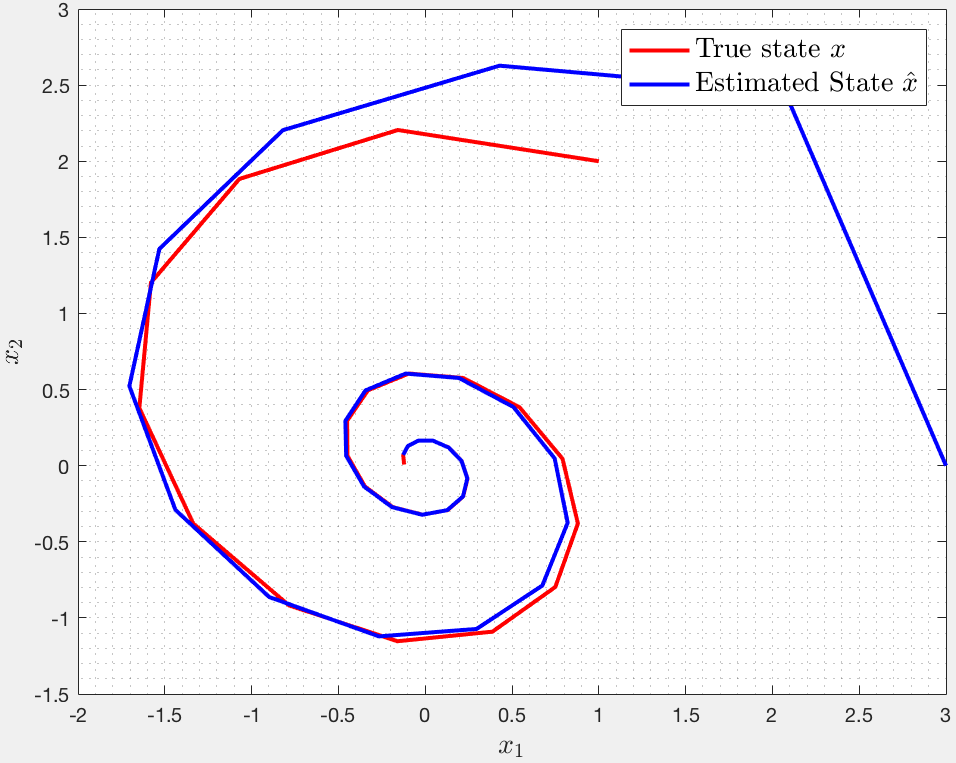
\includegraphics[width=\linewidth]{xest}
				\caption{State dynamics and estimation}
				\label{fig::xest}
			\end{minipage}
			\begin{minipage}{0.5\linewidth}
				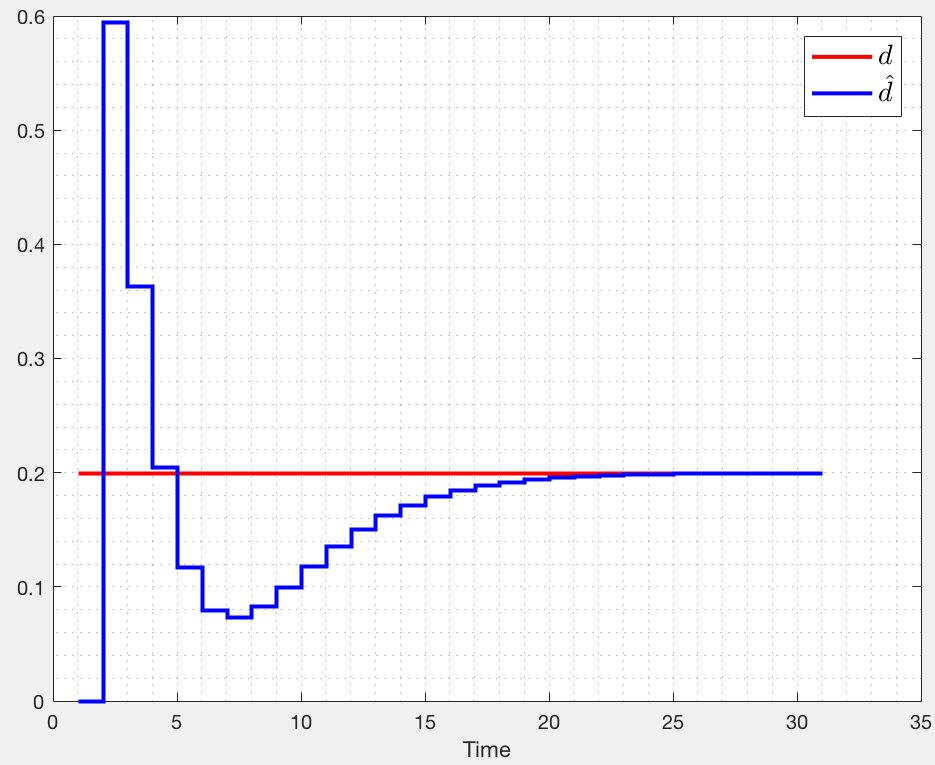
\includegraphics[width=0.95\linewidth]{dest}
				\caption{Disturbance estimation}
				\label{fig::dest}
			\end{minipage}
		\end{figure}
		
		\paragraph{} With such $L$, the error is steered to $0$ and we get \textbf{unbiased asymptotic estimators} for $x$ and $d$. With the Matlab command \texttt{place}, we can determine $L$ so that the resulting dynamics have given eigenvalues. Figures (\ref{fig::xest}) and (\ref{fig::dest}) show the convergence of $\hat{x}_k$ and $\hat{d}_k$ to their true values, with $u=0$ (the uncontrolled system is stable). In this example, we took the poles to be : 
		\begin{equation}
			\lambda_1 = 0.5, \quad \lambda_2 = 0.6, \quad \lambda_3 = 0.7
		\end{equation}
		
	}
\end{document}